\section{Data Pre-processing}
Preprocessing the data involves cleaning and organizing it to ensure accuracy, consistency, and ease of use. This step includes identifying and addressing duplicate entries, missing or incomplete data, and other inconsistencies. Proper preprocessing enhances the data's integrity, leading to more reliable results.\\

The dataset was imported into the workspace using the \texttt{read.csv()} function. To inspect the data, the first six lines were displayed using the \texttt{head()} function.\\

\begin{figure}[H]
    \begin{center}
    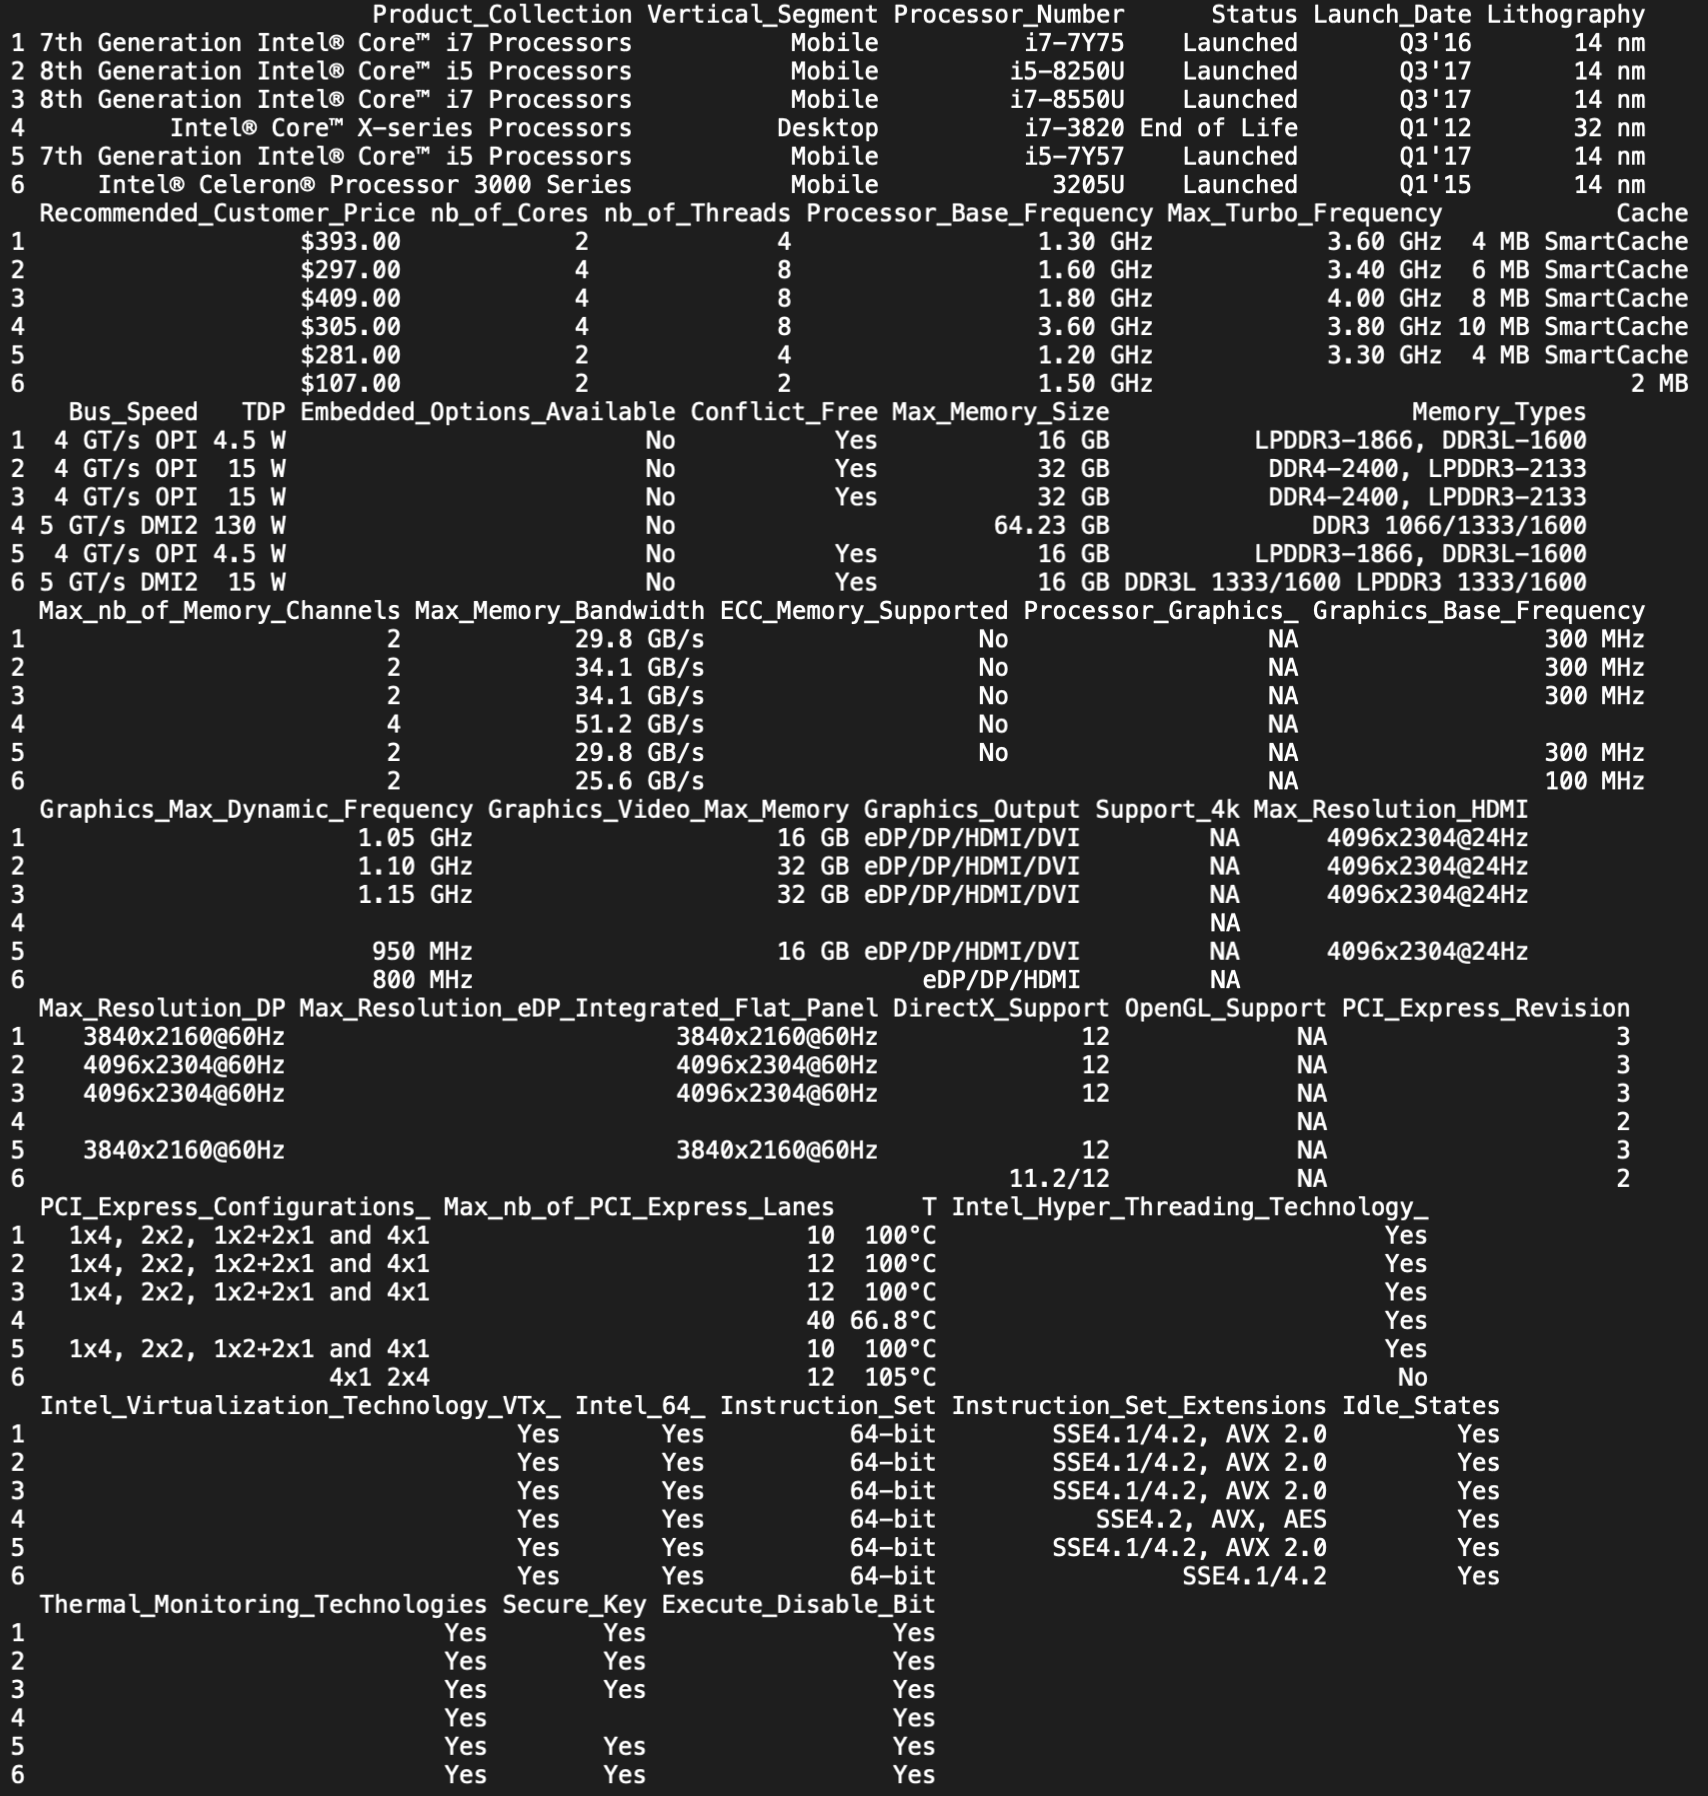
\includegraphics[width=14cm]{graphics/head.png}
    \end{center}
\end{figure}

After importing the data, it was summarized using the \texttt{vis\_dat()} function from the \texttt{visdat} library, which visualizes the data type of each attribute across all observations.

\begin{figure}[h]
    \centering
    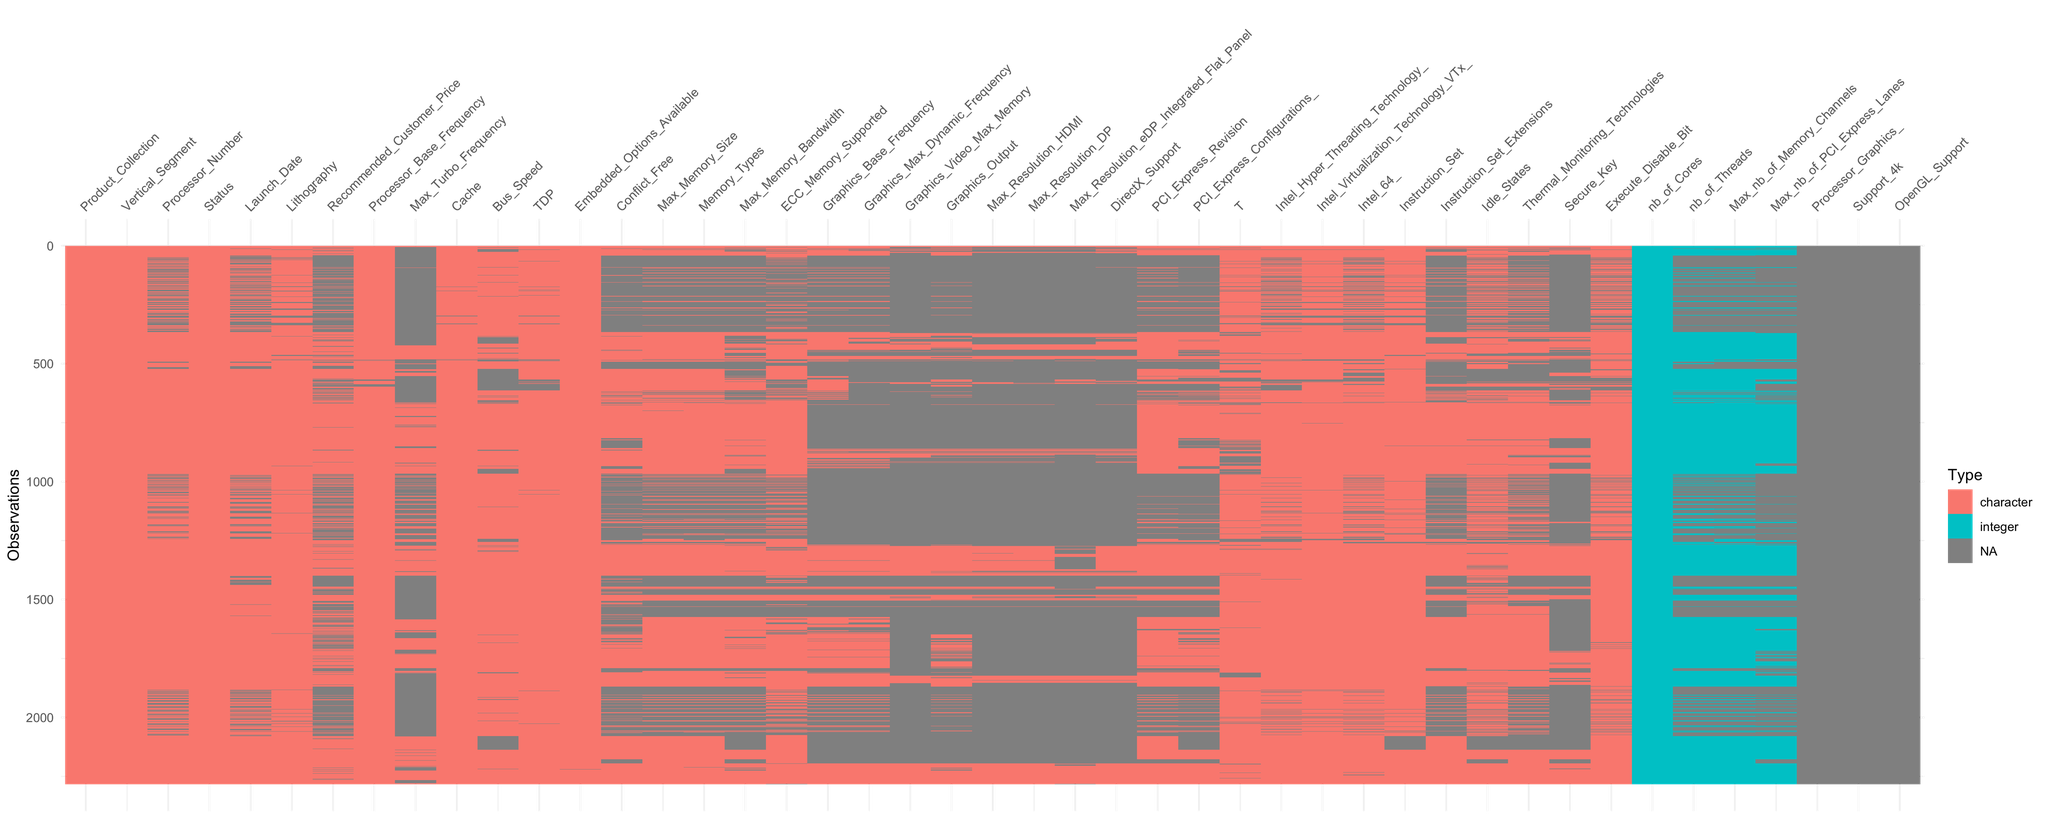
\includegraphics[width=16cm]{graphics/visdat.png}
    \caption*{Dataset visualization}
 \end{figure}

It can be seen that the dataset mostly consist of char types with some numeric features and a large of portion of data is missing. Therefore, to work with the dataset, feature selection followed by handling missing values has to be done and data transformation must take place in order to convert the char types into numeric for analyzing purposes.\\

\subsection{Missing values examination and attributes selection}

\begin{figure}[h]
    \centering
    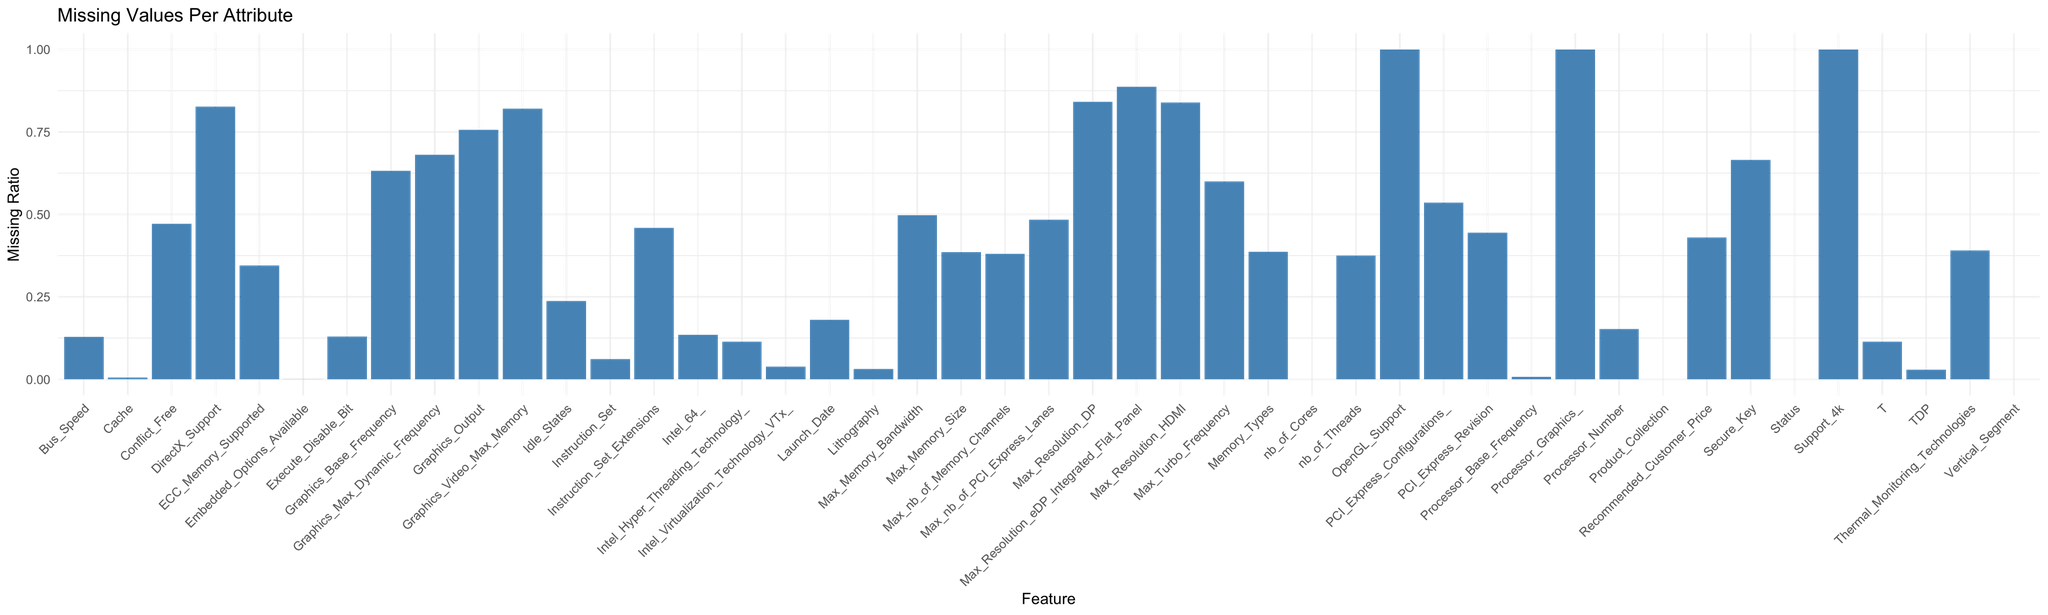
\includegraphics[width=16cm]{graphics/missingval.png}
    \caption*{Missing data ratio per attribute}
 \end{figure}

For further analysis, the attributes with less than 50\% of missing values are categorized into quintiles based on their missing value percentage ranges.

\begin{table}[H]
    \centering
    \begin{tabular}{|c|p{12cm}|}
        \hline
        \textbf{Category} & \textbf{Attributes} \\ \hline
        Less than 10\% & \texttt{Product\_Collection, Vertical\_Segment, Status, Lithography, nb\_of\_Cores, Processor\_Base\_Frequency, Cache, TDP, Embedded\_Options\_Available, Intel\_Virtualization\_Technology\_VTx, Instruction\_Set}\\ \hline

        10\% to 20\% & \texttt{Processor\_Number, Launch\_Date, Bus\_Speed, T, Intel\_Hyper\_Threading\_Technology, Intel\_64,'Execute\_Disable\_Bit} \\ \hline

        20\% to 30\% & \texttt{Idle\_States} \\ \hline

        30\% to 40\% & \texttt{nb\_of\_Threads, Max\_Memory\_Size, Memory\_Types, Max\_nb\_of\_Memory\_Channels, ECC\_Memory\_Supported, Thermal\_Monitoring\_Technologies} \\ \hline

        40\% to 50\% & \texttt{Recommended\_Customer\_Price, Conflict\_Free, Max\_Memory\_Bandwidth, PCI\_Express\_Revision, Max\_nb\_of\_PCI\_Express\_Lanes, Instruction\_Set\_Extensions} \\ \hline

        Above 50\% & Remaining attributes \\ \hline
    \end{tabular}
    \caption{Attributes categorization based on missing percentage}
\end{table}

\subsection{Data Relevance and Usefulness}
To ensure the integrity and robustness of our analysis, attributes with more than 50\% of absent information will be discarded. The others will be selected based on their relation to the base frequency of a CPU and the ratio of missing values. Specifically, the attributes of interest are:

\begin{itemize}
    \item \textbf{Processor\_Base\_Frequency}: This attribute represents the base clock speed of the CPU, measured in gigahertz (GHz). Higher base frequencies generally indicate faster processing capabilities and overall performance.
    \item \textbf{nb\_of\_Cores}: The number of cores in a CPU impacts its ability to handle multiple tasks simultaneously. CPUs with more cores can potentially support higher clock speeds under optimal conditions, affecting overall performance trends.
    \item \textbf{nb\_of\_Threads}: This attribute represents the number of threads supported by the CPU, which is often influenced by technologies like Intel's Hyper-Threading. A higher number of threads can contribute to better resource utilization and potentially higher effective clock speeds for certain workloads.
    \item \textbf{TDP (Thermal Design Power)}: The TDP indicates the maximum amount of heat the CPU cooling system needs to dissipate. This attribute is closely related to the CPU's power consumption and thermal characteristics, which can impact clock speed potential and performance.
    \item \textbf{Lithography}: This attribute refers to the manufacturing process node (e.g., 14nm, 10nm) used in producing the CPU. Advancements in manufacturing processes can lead to higher clock speeds and improved efficiency in newer CPU generations.
\end{itemize}

Our objective is to analyze historical trends in CPU clock speeds using these attributes. Understanding how clock speeds have evolved across different CPU generations, architectural improvements, and technological shifts is crucial for identifying patterns and making informed predictions. By focusing on these critical attributes, we aim to uncover insights into the factors driving CPU clock speed improvements and contributing to the overall technological progress in CPU development.\\

\subsection{Handling Missing Values}

To handle missing data, we employed median imputation. Although methods like listwise deletion, mean imputation, or regression imputation have their own merits, median imputation was chosen based on the following considerations:

\begin{itemize}
\item \textbf{Simplicity and Effectiveness}: Median imputation is straightforward to implement and often provides a better central tendency measure for skewed distributions compared to mean imputation.
\item \textbf{Neutral Algorithm}: Unlike regression imputation, which may introduce sample bias, median imputation does not assume a specific relationship between the missing values and other variables.
\item \textbf{Data Retention}: Removing rows with missing values (listwise deletion) would significantly shrink the size of our dataset. Median imputation allows us to retain as much data as possible while ensuring that the central tendency of the dataset is maintained.
\end{itemize}


\begin{lstlisting}[language=R]
    # Function to convert GHz to MHz if needed
    convert_units <- function(x) {
    if (str_detect(x, "GHz")) {
        value <- as.numeric(str_extract(x, "[0-9.]+")) * 1000
        return(value)
    }
    return(as.numeric(str_extract(x, "[0-9.]+")))
    }

    # Apply conversion and impute missing values with median
    data <- data %>%
    mutate(across(everything(), ~ {
        # Convert units if necessary and replace with numeric values
        . <- sapply(., function(cell) ifelse(is.na(cell) | cell == "", NA, convert_units(cell)))
        # Impute missing values with median
        . <- ifelse(is.na(.), median(., na.rm = TRUE), .)
        return(.)
    }))
\end{lstlisting}

The following \texttt{R} code handles the preprocessing of our dataset by converting units where necessary and imputing missing values with the median. The \texttt{convert\_units} function checks if the data contains "GHz" and converts it to "MHz" by multiplying the numeric value by 1000. This ensures uniformity in the measurement units. The mutate function from the \texttt{dplyr} package is used to apply these conversions across all columns of the dataset. For each cell, if the value is missing or empty, it is replaced with \texttt{NA}, then converted using the \texttt{convert\_units} function. Finally, any remaining \texttt{NA} values are imputed with the median of the respective column, ensuring the dataset remains complete and reliable for further analysis.


\newpage